% Fixture G7: hai mui ten chong nhau + mot ca cat vuong goc (hop le).
\documentclass[border=6pt]{standalone}
\usepackage{tikz}
\begin{document}
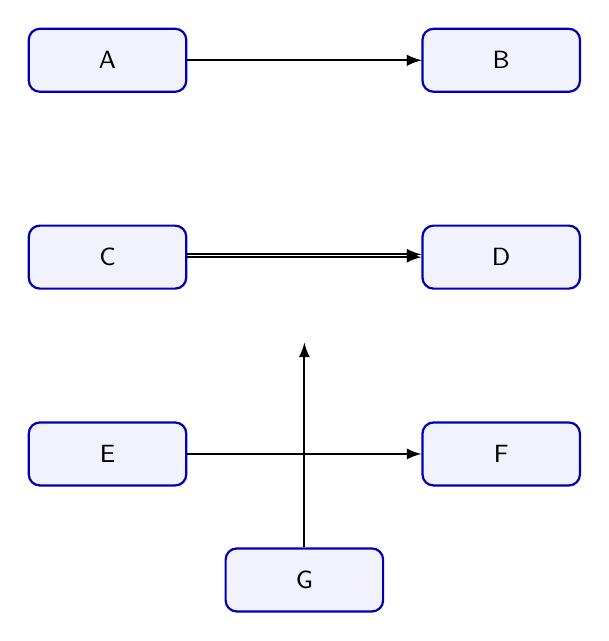
\begin{tikzpicture}[>=latex, font=\sffamily\small]
  \tikzstyle{blk}=[draw=blue!70!black, fill=blue!5, thick, rounded corners,
                   minimum width=2cm, minimum height=0.8cm, align=center]

  % --- CA 1: hai mui ten TRUNG KHIT (loi) ---
  \node[blk] (a1) at (0,0)   {A};
  \node[blk] (b1) at (5,0)   {B};
  \draw[->, thick] (a1.east) -- (b1.west);
  \draw[->, thick] (a1.east) -- (b1.west);

  % --- CA 2: hai mui ten SONG SONG cach ~1pt (loi) ---
  \node[blk] (a2) at (0,-2.5) {C};
  \node[blk] (b2) at (5,-2.5) {D};
  \draw[->, thick] (a2.east) -- (b2.west);
  \draw[->, thick] ([yshift=1pt]a2.east) -- ([yshift=1pt]b2.west);

  % --- CA 3: CAT VUONG GOC (hop le, khong duoc bao loi) ---
  \node[blk] (a3) at (0,-5)  {E};
  \node[blk] (b3) at (5,-5)  {F};
  \node[blk] (c3) at (2.5,-6.6) {G};
  \draw[->, thick] (a3.east) -- (b3.west);
  \draw[->, thick] (c3.north) -- ++(0,2.6);
\end{tikzpicture}
\end{document}
